\documentclass[11pt]{article}

\usepackage{fontenc} 
\usepackage{flushend} % last page balancing
\usepackage{geometry}
\geometry{
	paper=a4paper, % Change to letterpaper for US letter
	inner=2.5cm, % Inner margin
	outer=2.5cm, % Outer margin
	bindingoffset=0.0cm, % Binding offset - was 0.5
	top=1.5cm, % Top margin
	bottom=1.5cm, % Bottom margin
	% showframe, % Uncomment to show how the type block is set on the page
}
\usepackage{graphicx} % include figures
\usepackage[parfill]{parskip} % Tidy up layout
\usepackage[german]{babel}
\usepackage{csquotes}

\usepackage[
    backend=biber, 
    style=numeric,
    sorting=none,
    isbn=false
]{biblatex}
\addbibresource{literature.bib} % The filename of the bibliography

\renewcommand{\familydefault}{\sfdefault}

\begin{document}

%%%%%%%%%%%%%
% DECKBLATT %
%%%%%%%%%%%%%

\begin{titlepage}
\begin{center}

\vspace{-20mm}
\vspace*{20mm}

\begin{Huge}
\textbf{Das Heidelberger Institut für Geoinformationstechnologie gGmbH} \\ [18pt]
\end{Huge}

\begin{LARGE}
\textbf{in Kooperation mit der GIScience des \\ Geographischen Instituts Heidelberg} \\ [6pt]
\end{LARGE}

\vspace{50mm}

\begin{Large}
Bericht zur Wissenschaftlichen Hilfskraftstelle \\ [6pt]
im Zeitraum vom 01. November 2022 bis 30. September 2024
\end{Large}

\vspace{50mm}

\begin{table}[ht]
    \begin{center}
        \begin{tabular}{l l} 
        vorgelegt von: & Nikolaos Kolaxidis \\ [6pt]
        Studiengang: & M.Sc. Geographie \\ [6pt]
        Matrikelnummer: & 3694017 \\ [6pt]
        Email: & pd281@uni-heidelberg.de \\ [6pt]
        Betreuung: & Dr. Christina Ludwig \\
        \end{tabular}
    \end{center}
\end{table}

\vspace*{\fill}
\today

\end{center}
\end{titlepage}

\section{Das HeiGIT}

Das Heidelberger Institut für Geoinformationstechnologie gGmbH (HeiGIT) \autocite{HeiGIT2024}, wurde 2019 als gemeinnütziges An-Institut der Universität Heidelberg gegründet und wird von der Klaus Tschira Stiftung getragen. Es hat sich unter der wissenschaftlichen Leitung von Prof. Alexander Zipf auf die Entwicklung von Geoinformationstechnologien spezialisiert, mit dem Ziel, Gesellschaft und Umwelt durch Verbesserung von offenen Geoinformationen zu fördern. Als enger Kooperationspartner der GIScience Forschungsgruppe des Geographischen Instituts der Universität Heidelberg hat das HeiGIT den Anspruch, den Wissens- und Technologietransfer von grundlegender Forschung in Geoinformatik zu praktischen Anwendungen zu verbessern. Durch die enge Zusammenarbeit können HeiGIT und GIScience auf dem neuesten Stand der Technik bleiben und zukunftsweisende Ergebnisse von international anerkannter Qualität erzielen.

Das HeiGIT bietet Forschung und Entwicklung zur Unterstützung von Entscheidungsfindungen im Bereich nachhaltige Mobilität, humanitäre Hilfe und Klimaschutz. Dies wird durch offene Geoinformationen und open-source Software sowie der engen Zusammenarbeit mit ihren Partner*innen, die aus verschiedensten Bereichen kommen und auch die Gesellschaft als solche einschließt, erreicht. Nennenswerte direkte Kooperationspartner*innen sind das Deutsche Rote Kreuz und das Humanitarian OpenStreetMap Team, dazu zahlreiche indirekte wie Ärzte ohne Grenzen sowie viele Nationale Rotkreuz- und Rothalbmond-Gesellschaften. Regelmäßige Teilnahmen an internationalen geographischen und geoinformatischen Konferenzen wie der State of the Map, der AGILE und der FOSSGIS sowie Publikationen in namhaften Journals wie der Nature und dem ISPRS Journal of Photogrammetry and Remote Sensing, zeigen die hohe wissenschaftliche Relevanz und Qualität der Arbeit des HeiGIT. Zusätzlich ist das HeiGIT seit 2023 auch prominent auf Seiten rund um OpenStreetMap (OSM) genannt, da dieses aufgrund seiner Volunteered Geographic Information basierten und offenen Art stets eine wesentliche Rolle in den Forschungen und Produkten des HeiGIT spielt und das HeiGIT einige zentrale Produkte für den Umgang mit OSM entwickelt hat und bereitstellt.

Im HeiGIT sind vier sogenannte Fokusgruppen tägig, die sich mit verschiedenen zentralen Themenbereichen der Geoinformatik beschäftigen. Davon haben zwei eine eher technische Ausrichtung (Big Spatial Data Analytics \& Smart Mobililty) und zwei eine eher angewandte (Climate Action \& Geoinformation for Humanitarian Aid). 

\enquote{Big Spatial Data Analytics}, eine der zwei technischen Fokusgruppen, beschäftigen sich mit der Verarbeitung und Bereitstellung großer geoinformatischer Datenmengen, die bei Fernerkundung und OSM anfallen. Sie entwickeln Produkte zur Analyse und Visualisierung dieser Daten und liefern die nötige Software für die zwei angewandten Fokusgruppen. Ein Beispiel hierfür ist Ohsome \autocite{HeiGIT2024a}, welches die Abfrage von OSM-Daten vereinfacht und erweitert und weltweit zum Einsatz kommt.

\enquote{Climate Action} ist der neueste Zugang im HeiGIT und wurde aus dem Umstand heraus geschaffen, dass der Klimawandel einen immer größeren Stellenwert in den Projekten der anderen Fokusgruppen eingenommen und angepasste Produkte erfordert hat. Sie entwickeln Produkte zur Unterstützung von Klimaschutzmaßnahmen, die auf geoinformatischen Daten basieren, und erforschen Adaptions- und Mitigationsmöglichkeiten im Bezug zum Klimawandel auf kleinräumlicher und internationaler Ebene.

\enquote{Geoinformation for Humanitarian Aid} arbeiten eng mit humanitären Hilfsorganisationen zusammen und bieten Produkte zur Unterstützung von humanitären Maßnahmen an. Sie stellen den Kern des HeiGITs dar, da sie Geoinformationstechnologien für humanitäre Zwecke entwickeln und durch Veranstaltungen wie Mapathons und GIS-Kurse in entsprechenden Ländern den Wissenstransfer vorantreiben. Außerdem sind sie in Katastrophensituationen aktiv und helfen durch die Bereitstellung von Geoinformationsprodukten bei der Koordination von Hilfsmaßnahmen.

\enquote{Smart Mobility} entwickeln Produkte zur Unterstützung von nachhaltiger und inklusiver Mobilität und bieten mit dem OpenRouteService (ORS) \autocite{HeiGIT2024b} eine weltweit eingesetzte Routing-Engine zu Forschungszwecken an. Außerdem ermöglichen sie mit dessen Weiterentwicklung den beiden angewandten Fokusgruppen, Mobilität in Katastrophensituationen an entsprechenden Stellen zur Verfügung zu stellen und nachhaltige urbane Planung voranzutreiben.

Zudem sind viele Beschäftigte des HeiGIT auch in der Lehre tätig und bieten regelmäßig Seminare und Vorlesungen an, die sich an Studierende der Geographie und Geoinformatik richten. Dadurch wird der Wissenstransfer von der Forschung zurück in die Lehre gewährleistet und Studierende können frühzeitig in die Forschung eingebunden werden.

\section{Als WHK am HeiGIT}

Das HeiGIT bietet Studierenden verschiedener Fachrichtungen, aber vor Allem auch der Geoinformatik, die Möglichkeit, als Praktikant*in oder Wissenschaftliche Hilfskraft (WHK) in den verschiedenen Fokusgruppen oder im Rahmen bestimmter Projekte mitzuarbeiten. Auch internationale Studierende können am HeiGIT ein Praktikum absolvieren, was die Internationalität des HeiGITs unterstreicht.

Für Studierende der Geoinformatik ist eine Bewerbung durch die Nähe zum geographischen Studium meist nicht nötig. Vielmehr wird der Kontakt über Seminare sogar gerne gesucht, da in diesen bereits Kenntnisse und Leistungen gezeigt werden können, die im Grunde als Arbeitsproben verstanden werden können. Außerdem wird in diesem Rahmen oft die nötige Motivation zur Mitarbeit an geoinformatischen Themen evaluiert. Das familiäre Umfeld der Geographie in Heidelberg ermöglicht es, dass auf flachen Hierarchien Ideen ausgetauscht und Mitarbeiten in Projekten vereinbart werden können.

So bin ich auch an das Praktikum gekommen. In Seminaren wurde das HeiGIT immer wieder als Institution genannt und viele Fragestellungen und Methodiken, die in den Seminaren behandelt wurden, wurden in ähnlicher Weise auch im HeiGIT angewandt. So war es naheliegend, dass es nach einem Seminar mal eine Nachfrage bezüglich des HeiGIT gab, ob dort nach WHKs gesucht wird.

Ende 2022 begann im HeiGIT eine starke Expansionsphase, die das Team inklusive WHKs innerhalb anderthalb Jahre um fast das Doppelte hat wachsen lassen, was erst vor wenigen Monaten etwas stagniert ist. Daher war der Zeitpunkt perfekt für eine Stelle als WHK. Nach einem kurzen Austausch bezüglich Interessen und möglichen Projekten, an denen gearbeitet werden könnte, entschloss ich mich eine Stelle im Smart Mobility Team anzunehmen. Das war, wie sich anschließend herausstellte, genau die richtige Entscheidung. 

\subsection{Projekt HEAL}

Ursprünglich wurde ich zur Unterstützung des Projekts \enquote{Hitzeanpassung für vulnerable Bevölkerungsgruppen} (HEAL) \autocite{HEAL2024} eingestellt. Das Projekt zielt darauf ab, die steigende Gefahr von Hitzestress für vulnerable Bevölkerungsgruppen in Städten am Beispiel Heidelbergs zu untersuchen und zu mindern. Dies wird durch die Entwicklung einer hitzevermeidenden Routing-App erreicht, die auf dem ORS basiert. Die App kombiniert die individuellen Bedürfnisse hitzesensitiver Personen mit multimodalen Schattendaten, um hitzestressvermeidende Fußgänger*innenrouten zu wichtiger Infrastruktur zu bieten \autocite{Foshag.Furle.ea2024}.

Mein Part war das programmieren eines Tools zur Analyse des Routing-Algorithmus, welches in einem bestimmten Rahmen zufällige realistische Routen in Heidelberg generiert, die Alternativrouten zu vier Tageszeitpunkten mit den \enquote{normalen} Routen des ORS vergleicht und diverse Statistiken erstellt \autocite{HeiGIT2024e}. Dieses Tool sollte es ermöglichen, die Effektivität der hitzestressvermeidenden Routen sowie das Straßennetzwerk hinsichtlich Bereichen hohen Hitzestresses und wenigen Alternativen zu evaluieren und Verbesserungspotenziale sowohl für die App als auch für die Stadtplanung aufzuzeigen. Zur Veranschaulichung dient folgende Abbildung \ref{fig:HEAL}.

Die Mitarbeit an diesem Projekt hat meine Programmierkenntnisse massiv verbessert und mir inzwischen auch die Möglichkeit eröffnet, ein Paper in führender Autorenschaft zu dieser Thematik zu schreiben. Dies ist momentan in Arbeit und wird voraussichtlich Ende des Jahres 2024 veröffentlicht.

\subsection{Projekt SM2T}

Während des HEAL-Projektes kam ein weiteres Projekt hinzu, welches sich mit der Verbesserung der Fahrzeitmodellierung des ORS auf Grundlage von Social Media Daten beschäftigt. Das Projekt \enquote{Social Media 2 Traffic} (SM2T) \autocite{SM2T2024} versucht, Social Media Daten von der Plattform X (damals Twitter) und Uber zu sammeln und dafür zu nutzen, die Fahrzeitmodellierung des ORS mit realen Verkehrsdaten zu vergleichen. Hierzu wurde ein Paper veröffentlicht, an dem ich auch mitwirken durfte \autocite{Ludwig.Psotta.ea2023}. Meine Aufgabe war im Wesentlichen, wie in HEAL, eine Routen-Modellierung zu entwickeln, die die Fahrzeiten statistisch vergleicht und das beste Modell für die Fahrzeitmodellierung des ORS ermittelt \autocite{HeiGIT2023}.

Die Nennung im Paper als Co-Autor zeigte mir, dass das HeiGIT auch die Mitarbeit von WHKs hoch anerkennt, was ich aus bisherigen Berufserfahrungen so nicht kannte. Dies motivierte mich zusätzlich, mich in weitere Projekte einzubringen.

\begin{figure}[!h]
    \centering
    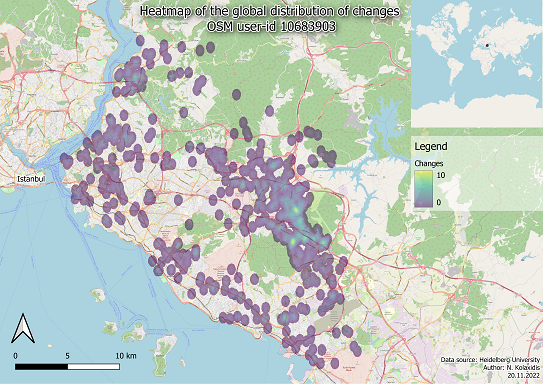
\includegraphics[width=0.8\textwidth]{figures/map.png}
    \caption{\emph{Vergleich einer abendlichen Alternativroute um 19 Uhr mit der normalen Route des ORS, aufgeteilt in einzelne Segmente (basierend auf OSM). Es ist zu sehen, dass die Alternative einen komplett anderen Verlauf hat und bei gerade mal 7 \% mehr Länge 58 \% weniger Hitzestress aufweist. Somit ist die Alternative als effektiv zu bewerten.}}
    \label{fig:HEAL}
\end{figure}

\subsection{ORS}

Mit der Zeit wurde ich in weitere kleinere Projekte und Aufgaben im Rahmen des Smart Mobility Teams, also im Wesentlichen rund um ORS, eingebunden. So habe ich beispielsweise ein Tutorial zum lokalen Bauen eines benutzerdefinierten Dockercontainers erstellt \autocite{HeiGIT2024d} oder auch ein QGIS-Modell, welches in einem Workshop für die AGILE Konferenz 2024 eine mögliche Nutzung des ORS zeigen soll. Insgesamt hat mir die WHK-Stelle einen guten Einblick in Arbeiten des HeiGIT und vor allem des Smart Mobility Teams gegeben.

\subsection{Projekte GIDL \& GeoWiKI}

Durch die Themenwahl meiner Masterarbeit und Eigeninteresse bin ich dann Anfang des Jahres einem weiteren Projekt zugestoßen, welches sich mit der Einbindung von geographischem Wissen in Machine Learning (\enquote{Geographically Informed Deep Learning} (GIDL)) beschäftigt und im Climate Action Team angesiedelt ist. Dies soll den hohen Energieverbrauch von Machine Learning Modellen auch in anderen Disziplinen reduzieren. Dazu wird ein bestehendes Land Use Land Cover (LULC) Deep Learning Modell, das LULC Utility \autocite{HeiGIT2024c}, angegangen und die Kostenfunktion mit Wahrscheinlichkeiten, basierend auf morphologischen und geographischen Metriken von LULC Flächen, angereichert. Das soll dazu führen, dass das Modell bestimmte Rahmenbedingungen, die wir als \enquote{realistisch} ansehen, nicht erst selber lernen muss und so schneller konvergiert, was zu einem geringeren Energieverbrauch führt. Zu diesem Thema ist momentan ein Paper in Arbeit, an dem ich als Co-Autor beteiligt bin. Mein Aufgabenbereich hierbei ist die Exploration verschiedener Metriken, die genutzt werden können, wie auch die Mitwirkung an der Implementierung und Evaluierung des Modells.

Basierend auf dieser Idee wurde darüber hinaus ein Projektproposal geschrieben, welches erst vor wenigen Wochen angenommen wurde und  ab Oktober 2024 startet. Das Projekt \enquote{Geographisches Wissen in Künstlicher Intelligenz} (GeoWiKI) soll erforschen, welche weiteren Möglichkeiten es gibt, geographisches Wissen in Deep Learning Modelle zu integrieren, um zum Einen die Modelle durch realistischere Vorhersagen zu verbessern und zum Anderen durch eine schnellere Modellkonvergenz den Energieverbrauch zu reduzieren. Also ein ähnliches Ziel wie das GIDL-Projekt, allerdings explorativer, unter Umständen auch durch Konzeption und Einbindung eines Graphenmodells und entsprechenden Ensemble-Learning-Methoden.

Im Rahmen dieses Projektes wird eine Stelle in der GIScience finanziert, für die ich auf Grundlage bisheriger Tätigkeiten in dem Bereich sowie großem Interesse und einer hohen Eigenmotivation angefragt wurde. Dadurch eröffnet sich für mich die Möglichkeit, auch nach dem Masterstudium im Kontext von HeiGIT und GIScience zu bleiben und an innovativen Ideen im Bereich der Geoinformatik zu forschen.

So endet Ende September meine Zeit als WHK am HeiGIT und ich werde ab Oktober 2024 in die GIScience wechseln, um dort an GeoWiKI zu forschen. Dafür bin ich dem HeiGIT, der GIScience und ganz besonders auch meiner Betreuerin Christina Ludwig sehr dankbar, die mir neben Alexander Zipf und Maciej Adamiak diese Möglichkeit eröffnet hat.

\subsection{Rund um den Job}

Zusätzlich zu allen Aufgaben, die im Rahmen der Projekte zu erledigen waren, konnte ich auch an diversen Meetings und Veranstaltungen des HeiGIT und der GIScience teilnehmen. Das schließt ebenfalls das monatliche Jour Fixe ein, in dem aktuelle Projekte und Entwicklungen beider Teams besprochen werden, sowie die regelmäßigen Mittagessen, Kaffeepausen und Feiern, in denen auch über nicht-arbeitsbezogene Themen gesprochen wird. Dadurch konnte ich das Team und die Arbeitsweise des HeiGIT besser kennenlernen und mich auch sozial in die Teams einbringen. 

\subsection{Das HeiGIT als Arbeitgeber}

Was im Zuge der angesprochenen Aktivitäten sehr positiv zu bemerken ist, ist die Wertschätzung, die den WHKs von den Mitarbeitenden entgegengebracht wird. Eigene Ideen werden ernst genommen und die Arbeit nicht als weniger wert abgestempelt, sondern als wichtiger Bestandteil des kompletten Unternehmens. Zudem sorgt diese Wertschätzung, aber auch die Offenheit, die Freundlichkeit und auch der Spaß an der Arbeit, für eine durchweg angenehme Arbeitsatmosphäre. Es ist stets zu spüren, dass die Arbeit einen Mehrwert für die Gesellschaft hat und die Menschen im HeiGIT und der GIScience ihre Ideen und Projekte um diesen zentralen Punkt herum aufbauen.

Außerdem sind alle Mitarbeitenden hilfsbereit und offen für Fragen und Anregungen. Es gibt immer die Möglichkeit, sich bei Problemen oder Unsicherheiten an Kolleg*innen zu wenden und um Hilfe zu bitten. Dadurch konnte ich auch in Projekten mitarbeiten, die nicht direkt in meinem Fachgebiet liegen und so meinen Horizont erweitern. Die Stelle und mögliche Praktika werden nach dem üblichen Stundensatz vergütet und die Arbeitszeiten sind flexibel, was es ermöglicht die Arbeit gut mit dem Studium zu vereinbaren.

Ein einziger Kritikpunkt ist, dass es durch die schnelle Expansion sowie die hohe Anzahl an Projekten und Mitarbeitenden manchmal schwer ist, den Überblick zu behalten. Das macht manchmal auch die Zusammenarbeit beider Institutionen schwierig, da es einer klaren Aufgabenteilung bedarf, diese aber häufig nicht gegeben ist. Es wird daher empfohlen, Offenheit mitzubringen und auch aktiv auf Kolleg*innen zugehen zu können. Ist dies gegeben, so ist das HeiGIT ein hervorragender Arbeitgeber, der einem viele Möglichkeiten bietet, sich zu entwickeln und zu entfalten.  

\section{Bezug zum Geographiestudium}

Durch meine Schwerpunktsetzung in der Geoinformatik ist die Arbeit am HeiGIT eine ideale Ergänzung zum Studium, da im Studium erworbene Kenntnisse direkt in der Praxis angewandt und vertieft werden können. Es gab zahlreiche Situationen, in denen eine am Morgen im Seminar erlernte Fähigkeit oder Methodik am Nachmittag unmittelbar in der Arbeit eingesetzt und erkannt werden konnte, welchen Mehrwert diese für die Praxis hat. Dadurch wirkte im Studium erlerntes, theoretisches Wissen wertvoller und greifbarer. Einige Seminare, die für die Praxis relevant waren, sind \enquote{FOSSGIS}, \enquote{(Advanced) Geoscripting} und \enquote{Geodatenbanken}, aber auch zum Beispiel \enquote{Time to Take Action} als Seminar des Geoinformation for Humanitarian Aid Teams, in dem die Arbeit des Teams und die Möglichkeiten von Geoinformationen im humanitären Kontext vorgestellt wurden.

Aber auch andersherum hat die Vertiefung in der Praxis und die Beschäftigung mit der Thematik das Studium einfacher gestaltet. Die Kombination von Theorie und Praxis hat mir geholfen, die Zusammenhänge besser zu verstehen und die Anwendungsmöglichkeiten besser einschätzen zu können. Dadurch fühlte sich ein Großteil der Arbeit an wie \enquote{bezahltes Lernen}, da neue Programmierkenntnisse, aktuelle Methodiken, tiefergehende theoretische Konstrukte und simpel gesagt Erfahrungen erworben werden konnten, die im Studium so nicht möglich gewesen wären.

Die Stelle hatte neben der fachlichen Weiterbildung und des \enquote{bezahlten Lernens} auch weitere Vorteile, die zuerst kaum ersichtlich waren. Zum Beispiel bieten das HeiGIT und die GIScience räumliche Möglichkeiten zum Arbeiten an, die für Studierende sonst nicht zugänglich sind. Durch regelmäßige Veranstaltungen im Team wie das Jour Fixe, aber auch gemeinsame soziale Aktivitäten wie Volleyball spielen und eben Mittagessen, kann das Verhältnis zu Dozierenden, Professor*innen sowie dem Kolleg*innenkreis gestärkt werden. Dadurch entstehen auch flachere Hierarchien, durch die Wege zwischen Studierenden und Professorium und Dozierenden stark verkürzt werden. Zudem wird so ein Einblick in aktuelle Forschung, Arbeitsweisen und die Sinnhaftigkeit von Seminarinhalten gegeben, der alles in allem das Studienleben in der Geographie stark bereichert.

Insgesamt hat die WHK-Stelle das Studien- und universitäre Leben stark vereinfacht und die Möglichkeit gegeben, sich bereits während des Studiums in einem professionellen Umfeld zu bewegen und zu entwickeln. Die Stelle in der GIScience im GeoWiKI-Projekt ist ein Sinnbild für die Wertschätzung, die WHKs im HeiGIT entgegengebracht wird.

\section{Fazit}

Das HeiGIT als Praktikums- oder WHK-Stelle ist empfehlenswert, absolut empfehlenswert! Die Arbeit ist abwechslungsreich, die Kolleg*innen sind freundlich und hilfsbereit, die Projekte spannend und die Wertschätzung, die einem entgegengebracht wird, enorm. Das HeiGIT hat mir gezeigt, dass die Geoinformatik und Geographie nicht nur interessante und vielfältige Themenfelder sind, sondern auch einen großen Mehrwert für die Gesellschaft haben können. Es hat mir gezeigt, dass ich in der Geoinformatik richtig bin und dass ich auch nach dem Studium in diesem Bereich arbeiten möchte. Damit hätte ich kaum eine bessere Stelle finden können, um mich auf das Berufsleben vorzubereiten.

\printbibliography

\end{document}